\newcommand{\sheetnum}{%
	06
}
%\setcounter{section}{\sheetnum-3}
\newcommand{\tutorialtitle}{%
    From the Vanishing Gradient Problem to Deep Learning
}
\newcommand{\tutorialtitleshort}{%
	Deep Learning
}
% for slides
\subtitle{\sheetnum \tutorialtitle}

%\maxdeadcycles=1000 % Workaround for ! Output loop---100 consecutive dead cycles because of too many figures

% The following use of algroithms does not work well with the notes:
%
%
%
%
% instead use the following for your algorithms:
%
%\begin{figure}[!t]
%\removelatexerror
%\begin{algorithm}[H]
    % your algo here
    %\label{alg:algolabel}
    %\caption{algocaption}
%\end{algorithm}
%\end{figure}
%\begin{algorithm}
% Below is the definition for the command \removelatexerror:
\makeatletter
\newcommand{\removelatexerror}{\let\@latex@error\@gobble}
\makeatother

\begin{document} %%%%%%%%%%%%%%%%%%%%%%%%%%%%%%%%%%%%%%%%%%%%%%%%%%%%%%%

\sheet{\sheetnum}{\tutorialtitleshort}

\ttopic{\tutorialtitle}

\columnratio{0.2,0.8}\textbf{}
\begin{paracol}{2}
%\setlength{\columnseprule}{0.1pt}
%\setlength{\columnsep}{5em}

\begin{rightcolumn}

% notes version will ignore it
\begin{frame}
\titlepage
\end{frame}

%\mode<presentation>{
%\begin{frame}
%\begin{center} \huge
    %Hopping onto the Deep Learning Bandwagon
%\end{center}
%\end{frame}
%}


\begin{frame}
\tableofcontents
\end{frame}


\mode<all>
\section{The Vanishing Gradient Problem}

% -----------------------------------------------------------------------------
\begin{frame}\frametitle{\secname}
	\begin{center}
		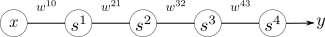
\includegraphics[width=10cm]{img/simple_arch}
	\end{center}
    forward pass
    \begin{align}
    y\;\;&=\;\;
    f(h^{4})\\
    \;\;&=\;\;
    f\big(w^{43} \cdot f(h^{3})\big)\\
    \;\;&=\;\;
    f\Big(w^{43} f\big(w^{32} \cdot f(h^{2})\big)\Big)\\
    \;\;&=\;\;
    f\bigg(w^{43} f\Big(w^{32} \cdot f\big(w^{21} \cdot f(h^{1})\big)\Big)\bigg)\\
    \;\;&=\;\;
    f\bigg(w^{43} f\Big(w^{32} \cdot f\big(w^{21} \cdot f(w^{10} \cdot x)\big)\Big)\bigg)
    \end{align}
\end{frame}

% -----------------------------------------------------------------------------
\begin{frame}\frametitle{\secname}
	\begin{center}
		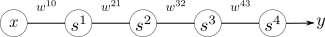
\includegraphics[width=10cm]{img/simple_arch}
	\end{center}
    backward pass:
    \begin{align}
     \frac{\partial y}{\partial w^{10}}
     \;\;&\stackrel{\mathclap{
    \substack{\text{chain}\\ \text{rule}}}
    }{=}\;\;
    \frac{\partial y}{\partial h^{1}}
    \cdot \frac{\partial h^1}{\partial w^{10}}\\
    \;\;&=\;\;
    \frac{\partial y}{\partial h^{2}}
    \cdot \frac{\partial h^{2}}{\partial h^{1}}
    \cdot \frac{\partial h^1}{\partial w^{10}}\\
    \;\;&=\;\;
    \frac{\partial y}{\partial h^{3}}
    \cdot \frac{\partial h^{3}}{\partial h^{2}}
    \cdot \frac{\partial h^{2}}{\partial h^{1}}
    \cdot \frac{\partial h^1}{\partial w^{10}}\\
    \;\;&=\;\;
    \frac{\partial y}{\partial h^{4}}
    \cdot \frac{\partial h^{4}}{\partial h^{3}}
    \cdot \frac{\partial h^{3}}{\partial h^{2}}
    \cdot \frac{\partial h^{2}}{\partial h^{1}}
    \cdot \frac{\partial h^1}{\partial w^{10}}\\
    \;\;&=\;\;
    =f'(h^{4}) w^{43} \cdot f'(h^{3}) w^{32} \cdot f'(h^{2}) w^{21} \cdot f'(h^{1}) w^{10}
    \end{align}
\end{frame}



\mode*

\clearpage

\end{rightcolumn}
\end{paracol}

\end{document}
